%%%%%%%%%%%%%%%%%%%%%%%%%%%%%%%%%%%%%%%%%%%%%%%%%%%%%%%%%%%%%%%%%%%%%%%%%%%%%%%%%%
\begin{frame}[fragile]\frametitle{}
\begin{center}
{\Large Tic-Tac-Toe}
\end{center}
\end{frame}


%%%%%%%%%%%%%%%%%%%%%%%%%%%%%%%%%%%%%%%%%%%%%%%%%%%%%%%%%%%%%%%%%%%%%%%%%%%%%%%%%%
\begin{frame}[fragile]\frametitle{Introduction}


\begin{columns}
\begin{column}{0.5\textwidth}
\begin{itemize}
\item Popular, small, childhood game
\item Known states, agent, environment and reward, easy to imagine and codify
\item Many variants though:
	\begin{itemize}
	\item X-O : each player aims to place three of their marks in a horizontal, vertical, or diagonal row in a 3x3 grid. 
	\item Numeric: In the 3x3 grid, numbers 1 to 9 are filled, with one number in each cell. The first player plays with the odd numbers, the second player plays with the even numbers, i.e. player 1 can enter only an odd number in the cell while player 2 can enter an even number in one of the remaining cells. Each number can be used exactly once in the entire grid. The player who puts down 15 points in a line - (column, row or a diagonal) wins the game.
	
	{\tiny (Ref: Tic-Tac-Toe Classical-RL - Prateek Ralhan)}
	\end{itemize}
\end{itemize}

\end{column}
\begin{column}{0.5\textwidth}  %%<--- here
\begin{center}
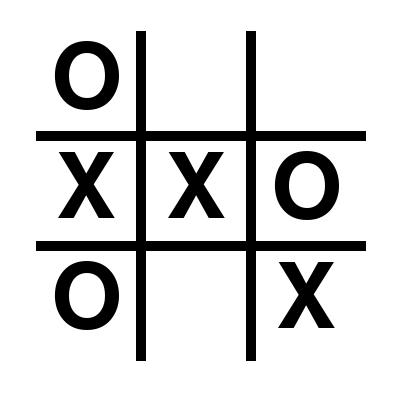
\includegraphics[width=0.8\linewidth,keepaspectratio]{rl70}
\end{center}
\end{column}
\end{columns}

\end{frame}

%%%%%%%%%%%%%%%%%%%%%%%%%%%%%%%%%%%%%%%%%%%%%%%%%%%%%%%%%%%%%%%%%%%%%%%%%%%%%%%%%
\begin{frame}[fragile]\frametitle{Min Max Algorithm}


\begin{columns}
\begin{column}{0.5\textwidth}
\begin{itemize}
\item Consider a game which has 4 final states and paths to reach final state are from root to 4 leaves of a perfect binary tree as shown.
\item Assume you are the maximizing player and you get the first chance to move, i.e., you are at the root and your opponent at next level. 
\item Which move you would make as a maximizing player considering that your opponent also plays optimally?
\end{itemize}

\end{column}
\begin{column}{0.5\textwidth}  %%<--- here
\begin{center}
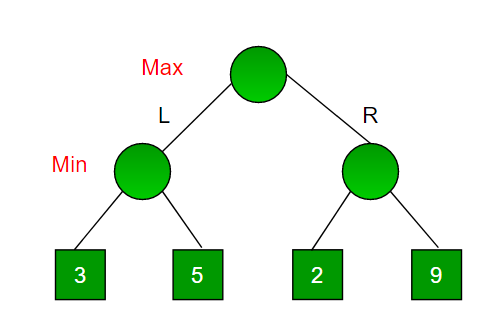
\includegraphics[width=0.8\linewidth,keepaspectratio]{rl71}
\end{center}
\end{column}
\end{columns}

{\tiny (Ref: Minimax Algorithm in Game Theory - Geek For Geeks)}

\end{frame}

%%%%%%%%%%%%%%%%%%%%%%%%%%%%%%%%%%%%%%%%%%%%%%%%%%%%%%%%%%%%%%%%%%%%%%%%%%%%%%%%%
\begin{frame}[fragile]\frametitle{Min Max Algorithm}


\begin{columns}
\begin{column}{0.5\textwidth}
\begin{itemize}
\item This is a backtracking based algorithm, it tries all possible moves, then backtracks and makes a decision. 
\item Maximizer goes LEFT: It is now the minimizers turn. The minimizer now has a choice between 3 and 5. Being the minimizer it will definitely choose the least among both, that is 3
\item Maximizer goes RIGHT: It is now the minimizers turn. The minimizer now has a choice between 2 and 9. He will choose 2 as it is the least among the two values.
\end{itemize}

\end{column}
\begin{column}{0.5\textwidth}  %%<--- here
\begin{center}
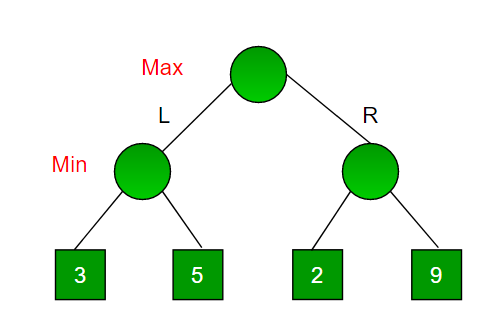
\includegraphics[width=0.8\linewidth,keepaspectratio]{rl71}
\end{center}
\end{column}
\end{columns}

{\tiny (Ref: Minimax Algorithm in Game Theory - Geek For Geeks)}

\end{frame}

%%%%%%%%%%%%%%%%%%%%%%%%%%%%%%%%%%%%%%%%%%%%%%%%%%%%%%%%%%%%%%%%%%%%%%%%%%%%%%%%%
\begin{frame}[fragile]\frametitle{Min Max Algorithm}


\begin{columns}
\begin{column}{0.5\textwidth}
\begin{itemize}
\item Being the maximizer you would choose the larger value that is 3. 
\item Hence the optimal move for the maximizer is to go LEFT and the optimal value is 3.
\end{itemize}

\end{column}
\begin{column}{0.5\textwidth}  %%<--- here
\begin{center}
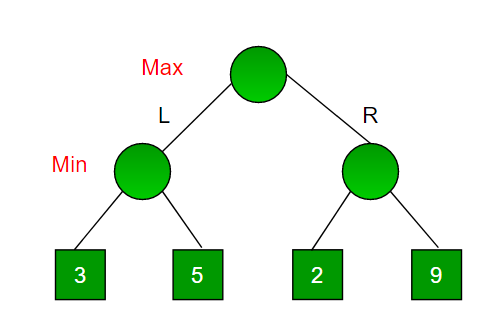
\includegraphics[width=0.8\linewidth,keepaspectratio]{rl71}
\end{center}
\end{column}
\end{columns}

{\tiny (Ref: Minimax Algorithm in Game Theory - Geek For Geeks)}

\end{frame}

%%%%%%%%%%%%%%%%%%%%%%%%%%%%%%%%%%%%%%%%%%%%%%%%%%%%%%%%%%%%%%%%%%%%%%%%%%%%%%%%%
\begin{frame}[fragile]\frametitle{Min Max Tic Tac Toe}


\begin{columns}
\begin{column}{0.5\textwidth}
\begin{itemize}
\item In Tic Tac Toe, in the middle of the games, say, here is the board position
\item Here, of the three possible moves available to player X
\item  ‘X’ in the center square is the only action that leads to a winning outcome
\item Note that Player X makes Move 1, Player Y makes Move 2 and Player X makes Move 3. This mini-game can end as early as after Move 1.
\end{itemize}

\end{column}
\begin{column}{0.5\textwidth}  %%<--- here
\begin{center}
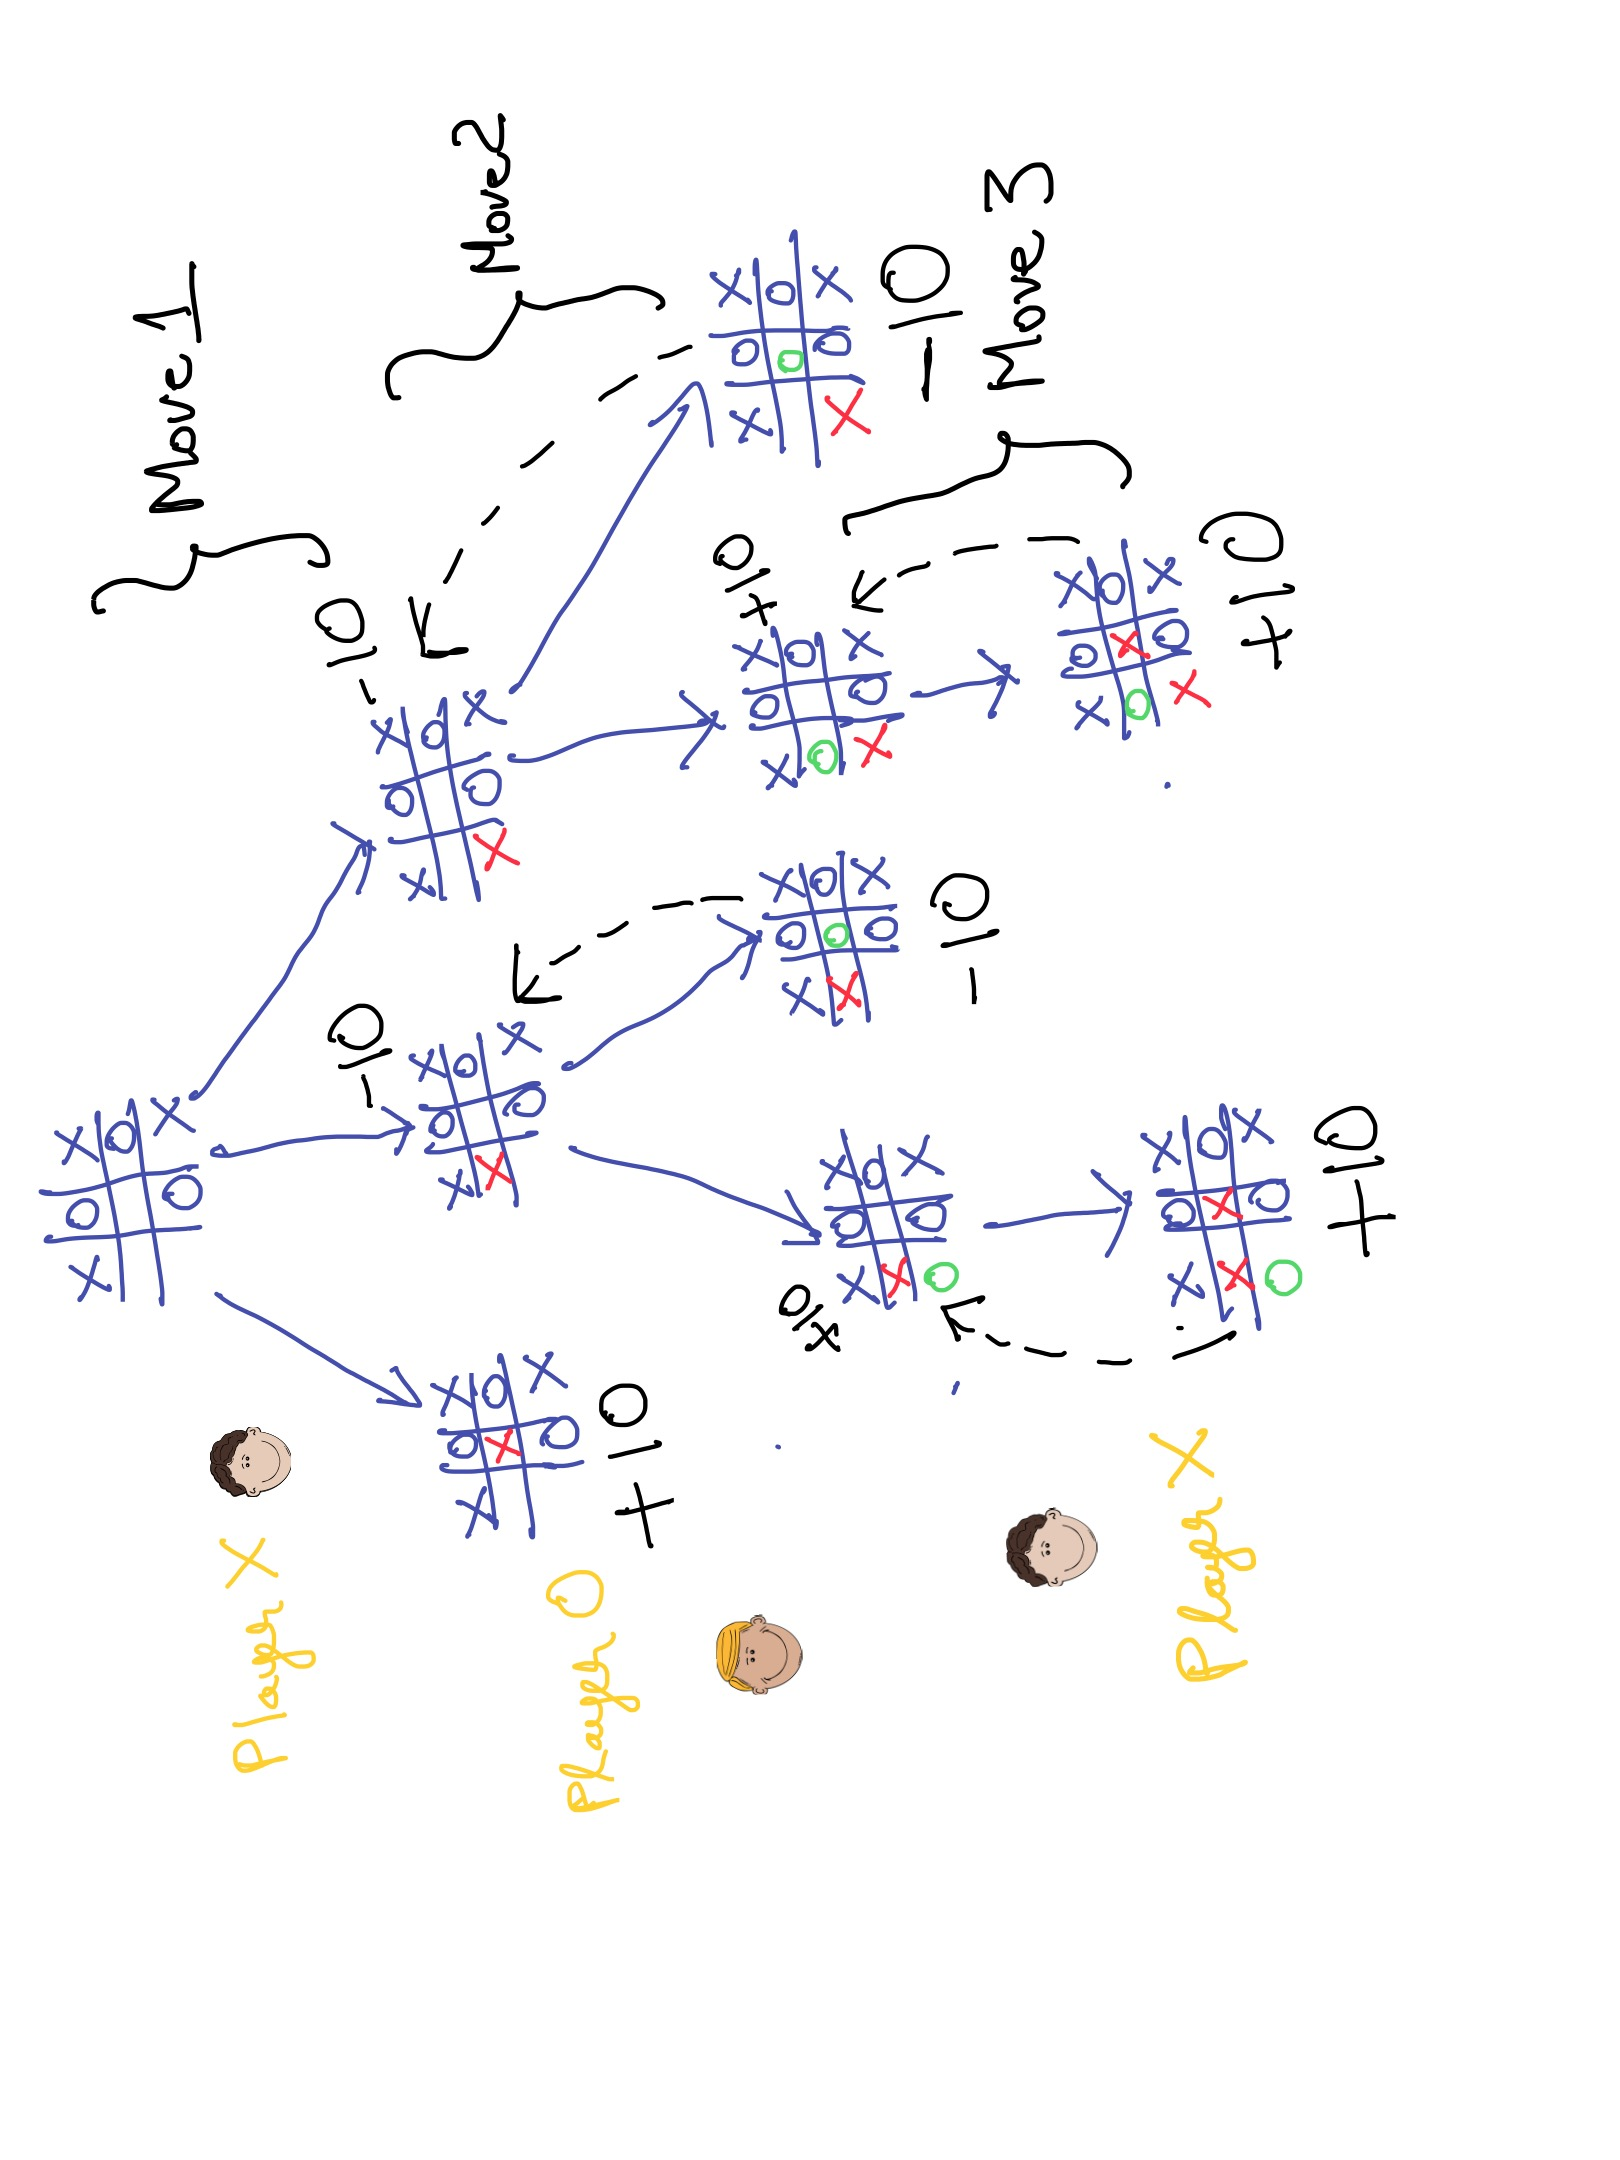
\includegraphics[width=0.8\linewidth,keepaspectratio]{rl72}
\end{center}
\end{column}
\end{columns}

{\tiny (Ref: Solving Tic-Tac-Toe with Minimax - Govind G Nair)}

\end{frame}

%%%%%%%%%%%%%%%%%%%%%%%%%%%%%%%%%%%%%%%%%%%%%%%%%%%%%%%%%%%%%%%%%%%%%%%%%%%%%%%%%
\begin{frame}[fragile]\frametitle{Min Max Tic Tac Toe}



\begin{center}
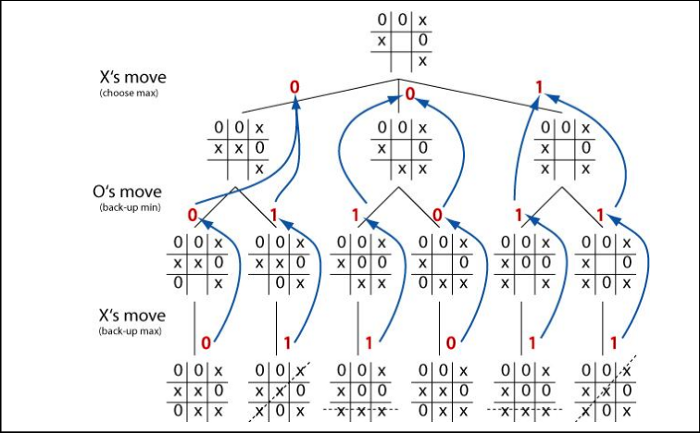
\includegraphics[width=0.8\linewidth,keepaspectratio]{rl74}
\end{center}

Evident that taking move on the right at next level is beneficial.

{\tiny (Ref: Playing Tic Tac Toe using Reinforcement Learning - Rohit Agarwal)}

\end{frame}



% %%%%%%%%%%%%%%%%%%%%%%%%%%%%%%%%%%%%%%%%%%%%%%%%%%%%%%%%%%%%%%%%%%%%%%%%%%%%%%%%%
% \begin{frame}[fragile]\frametitle{RL Tic Tac Toe}


% \begin{columns}
% \begin{column}{0.5\textwidth}
% \begin{itemize}
% \item 
% \end{itemize}

% \end{column}
% \begin{column}{0.5\textwidth}  %%<--- here
% \begin{center}
% 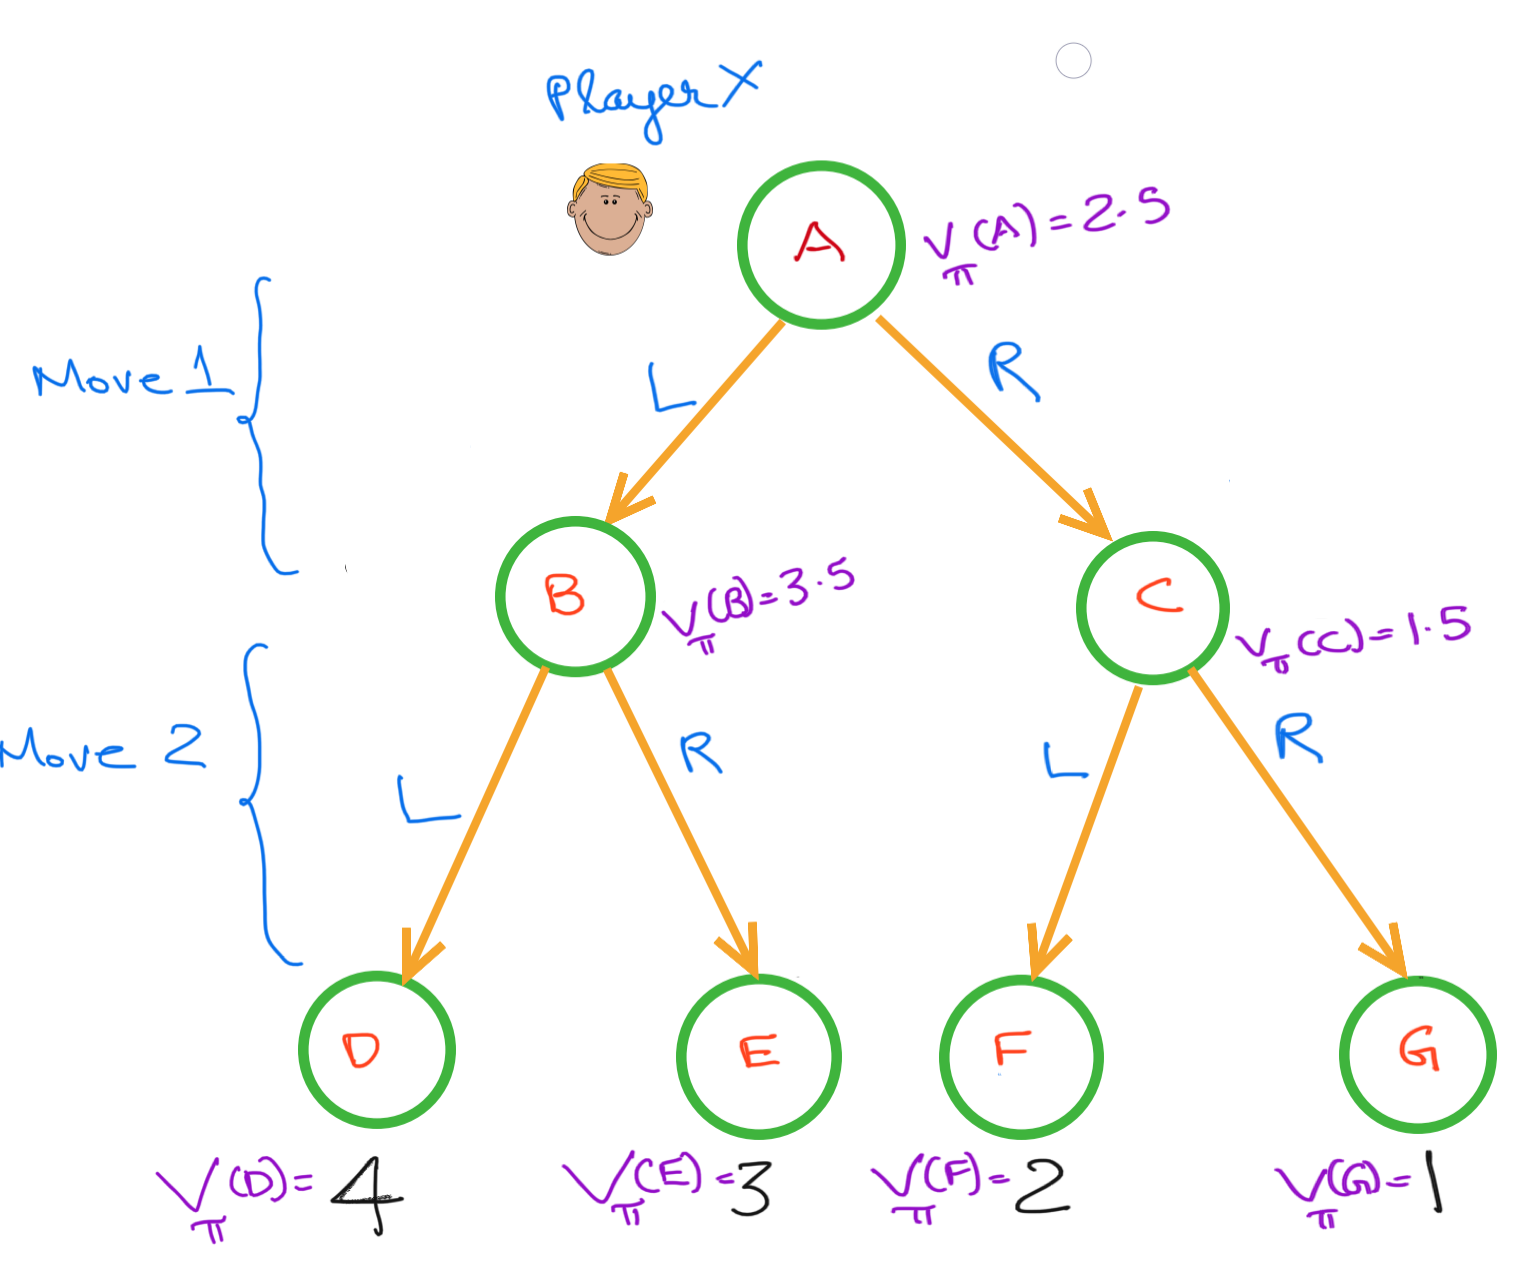
\includegraphics[width=0.8\linewidth,keepaspectratio]{rl73}
% \end{center}
% \end{column}
% \end{columns}

% {\tiny (Ref: Solving Tic-Tac-Toe with Reinforcement Learning - Govind G Nair)}

% \end{frame}


